\documentclass[aspectratio=169,11pt]{beamer}
\usepackage{beamerucad}
\usepackage{amssymb}
\usepackage{listings}
\definecolor{ckw}{HTML}{2563AB}\definecolor{cst}{HTML}{2E8B57}\definecolor{ccm}{HTML}{8A8F98}
\lstdefinestyle{py}{language=Python,basicstyle=\ttfamily\footnotesize,
 keywordstyle=\color{ckw}\bfseries,stringstyle=\color{cst},commentstyle=\color{ccm}\itshape,
 showstringspaces=false,columns=fullflexible,keepspaces=true,
 backgroundcolor=\color{ucadband!8},frame=leftline,framerule=2.5pt,rulecolor=\color{ucadband},
 xleftmargin=8pt,aboveskip=3pt,belowskip=1pt,basewidth=0.5em}
\lstset{style=py}
\title{Introduction au ML — Séance 6}
\subtitle{Classifier pour de vrai : régression logistique, seuil et métriques honnêtes}
\author{Dr. El Hadji Bassirou TOURÉ}
\institute{Département de Mathématiques et Informatique\\ Faculté des Sciences et Techniques\\ Université Cheikh Anta Diop de Dakar}
\date{}
\setucadfoot{Introduction au ML --- Séance 6 \quad\textbullet\quad Dr. El Hadji Bassirou TOURÉ --- DMI/FST/UCAD}
\graphicspath{{figs/}}
\begin{document}

\begin{frame}[plain,noframenumbering]\titlepage\end{frame}

\begin{frame}{Objectifs de la séance}
\begin{ucaddef}[Contenu]
{\small Cette séance reprend la classification là où les Séances 3 et 5 ont buté : prédire le \textbf{paludisme}, présent chez $11{,}8\,\%$ des patients seulement. Elle introduit le bon modèle — la \textbf{régression logistique} — et surtout les bons instruments de mesure.}
\end{ucaddef}
\begin{itemize}\small
  \item Transformer un score linéaire en \textbf{probabilité} : la sigmoïde, la régression logistique, la \textbf{log-loss}.
  \item Décomposer les erreurs : la \textbf{matrice de confusion}, \textbf{precision}, \textbf{recall}, \textbf{F1}.
  \item Le \textbf{seuil} de décision comme curseur — et non comme constante universelle.
  \item Juger le classement lui-même : la courbe \textbf{ROC} construite à la main, l'\textbf{AUC}.
  \item Le \textbf{déséquilibre de classes} : pourquoi l'accuracy ment, et quelles métriques disent la vérité.
\end{itemize}
\end{frame}

% #####################################################################
\section{Reprendre le problème du paludisme}

\begin{frame}{Là où la Séance 5 s'est arrêtée}
\begin{ucadfront}[Le constat du mini-défi]
{\small La régression linéaire, appliquée à la cible paludisme $\in \{0,1\}$, produit des sorties entre $0{,}008$ et $0{,}248$ — ni bornées, ni interprétables. Seuillées à $0{,}5$ : \textbf{zéro positif prédit}, accuracy $0{,}8825$, soit exactement la baseline « personne n'a le paludisme ». L'arbre de la Séance 3 avait échoué au même endroit.}
\end{ucadfront}
{\small Deux choses manquent : un modèle dont la sortie est une vraie \textbf{probabilité} — et des \textbf{métriques} capables de voir une classe rare. La séance construit les deux, dans cet ordre.}
\end{frame}

% #####################################################################
\section{La régression logistique}

\begin{frame}{L'idée : un score linéaire passé au variateur}
\begin{ucadfront}[Analogie]
{\small Un variateur de lumière : tourné très à gauche, la pièce est éteinte ; très à droite, pleinement allumée ; entre les deux, toutes les nuances. La régression logistique garde la somme pondérée des Séances 5 — le \emph{score} — et la passe dans un variateur : très négatif $\to$ probabilité proche de $0$, très positif $\to$ proche de $1$, autour de zéro $\to$ la pénombre du doute.}
\end{ucadfront}
\begin{ucaddef}[L'idée en une phrase]
{\small La \textbf{régression logistique} est le modèle linéaire de la Séance 5, suivi d'une fonction qui écrase le score dans $]0,1[$ pour en faire une \textbf{probabilité} d'appartenir à la classe $1$.}
\end{ucaddef}
\end{frame}

\begin{frame}{La sigmoïde, formellement}
\begin{ucaddef}[Définition]
{\small La \textbf{sigmoïde} transforme tout réel $z$ en un nombre de $]0,1[$, de façon croissante et symétrique autour de $\sigma(0) = 0{,}5$.}
\end{ucaddef}
\ucadformula{\sigma(z) \;=\; \frac{1}{1 + e^{-z}}}
{\small (Rappel : $e^{-z}$ est énorme quand $z$ est très négatif, quasi nul quand $z$ est très positif.) Donc $\sigma(z) \to 0$ en $-\infty$, $\to 1$ en $+\infty$ — sans jamais sortir de l'intervalle, contrairement à la droite nue de la Séance 5.}
\centering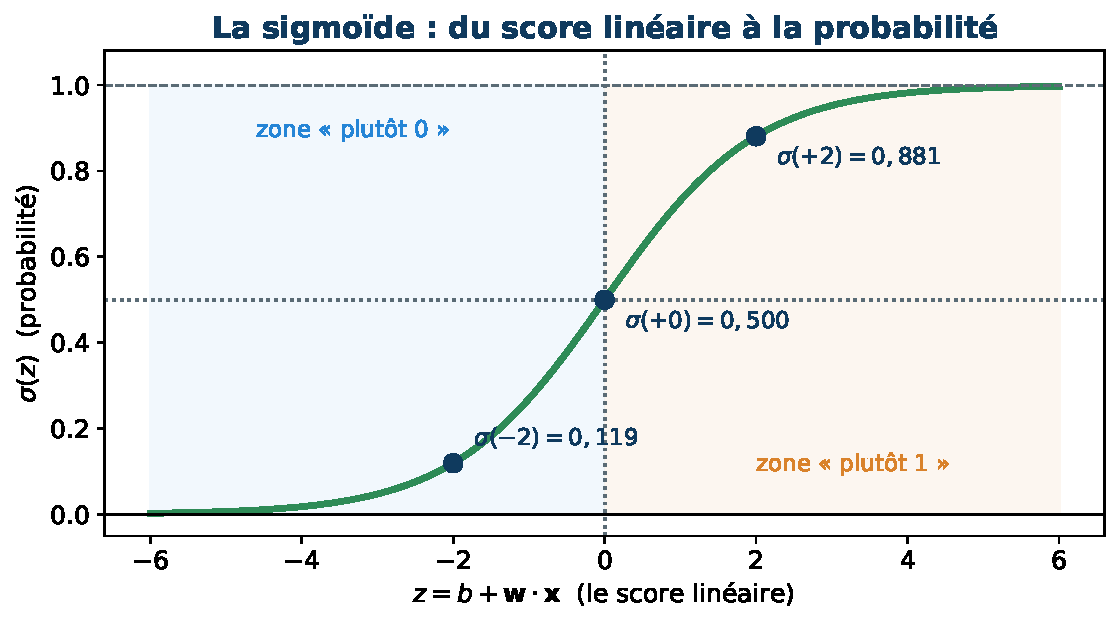
\includegraphics[width=0.36\linewidth]{f6_sigmoid}
\end{frame}

\begin{frame}{Exemple — la sigmoïde en chiffres}
\begin{ucadex}[Cinq scores et leurs probabilités]
{\small \begin{center}\renewcommand{\arraystretch}{1.05}\begin{tabular}{c|ccccc}
score $z$ & $-4$ & $-2$ & $0$ & $+2$ & $+4$\\\hline
$\sigma(z)$ & $0{,}018$ & $0{,}119$ & $0{,}500$ & $0{,}881$ & $0{,}982$\\
\end{tabular}\end{center}
Deux symétries à retenir : $\sigma(-z) = 1 - \sigma(z)$ (les lignes $-2$ et $+2$ se répondent), et $z = 0$ est l'exact point d'indécision. Quatre unités de score suffisent à passer de « presque sûrement non » à « presque sûrement oui ».}
\end{ucadex}
\end{frame}

\begin{frame}{Le modèle logistique, formellement}
\begin{ucaddef}[Définition]
{\small La \textbf{régression logistique} prédit la probabilité de la classe $1$ en passant le score linéaire dans la sigmoïde, puis décide en comparant cette probabilité à un \textbf{seuil} $s$.}
\end{ucaddef}
\ucadformula{\hat p \;=\; \sigma\big(b + \mathbf{w}\cdot\mathbf{x}\big) \;\in\; ]0,1[\,, \qquad \hat y \;=\; \mathbf{1}\big[\hat p \geq s\big] \quad (s = 0{,}5 \text{ par défaut})}
{\small Mêmes paramètres qu'en Séance 5 — un poids par variable, un intercept — mais la sortie a changé de nature : $\hat p$ est une probabilité, et la \emph{décision} $\hat y$ est une étape séparée, gouvernée par $s$. Cette séparation prédire/décider est le cœur de toute la séance. Malgré son nom, la régression logistique est un modèle de \textbf{classification}.}
\end{frame}

\begin{frame}{Exemple — un patient terme à terme}
\begin{ucadex}[Le modèle du paludisme évalue une patiente]
{\small Modèle entraîné sur DataSANTÉ-221 (variables \emph{standardisées}, Séance 4) : $b = -2{,}238$ et
\begin{center}\footnotesize\renewcommand{\arraystretch}{1.05}\begin{tabular}{l|ccccc}
 & âge & glycémie & hémoglobine & fièvre & saison\\\hline
poids $w_j$ & $0{,}02$ & $-0{,}10$ & $0{,}04$ & $0{,}12$ & $0{,}75$\\
$x$ standardisé & $-0{,}17$ & $-1{,}95$ & $1{,}40$ & $0{,}90$ & $1{,}12$\\
\end{tabular}\end{center}
$z = -2{,}238 + 0{,}02\!\cdot\!(-0{,}17) - 0{,}10\!\cdot\!(-1{,}95) + 0{,}04\!\cdot\!1{,}40 + 0{,}12\!\cdot\!0{,}90 + 0{,}75\!\cdot\!1{,}12 = \mathbf{-1{,}03}$\\[2pt]
$\hat p = \sigma(-1{,}03) = \mathbf{0{,}264}$. À seuil $0{,}5$ : prédiction $\hat y = 0$ — alors que cette patiente \emph{a} le paludisme ($y = 1$). Retenir ce cas : il reviendra.}
\end{ucadex}
\end{frame}

\begin{frame}{Exemple — un second patient, clairement négatif}
\begin{ucadex}[Un bien-portant de la saison sèche]
{\small Même modèle, une autre patiente — saison sèche, fièvre basse :
\begin{center}\footnotesize\renewcommand{\arraystretch}{1.05}\begin{tabular}{l|ccccc}
 & âge & glycémie & hémoglobine & fièvre & saison\\\hline
poids $w_j$ & $0{,}02$ & $-0{,}10$ & $0{,}04$ & $0{,}12$ & $0{,}75$\\
$x$ standardisé & $+0{,}50$ & $+0{,}30$ & $-0{,}50$ & $-1{,}00$ & $-0{,}90$\\
\end{tabular}\end{center}
$z = -2{,}238 + 0{,}01 - 0{,}03 - 0{,}02 - 0{,}12 - 0{,}675 = \mathbf{-3{,}07}$, donc $\hat p = \sigma(-3{,}07) = \mathbf{0{,}044}$. Le terme de saison ($-0{,}675$) écrase tous les autres : hors hivernage, le modèle est \emph{confiant} qu'il n'y a pas de paludisme. Décision $\hat y = 0$ à tout seuil raisonnable — et cette fois, à juste titre. Comparé à la patiente précédente ($\hat p = 0{,}264$), on voit le modèle \textbf{trier} : il donne bien plus de probabilité aux vrais malades.}
\end{ucadex}
\end{frame}

\begin{frame}{Lire les coefficients : le sens avant tout}
\begin{ucaddef}[L'idée en une phrase]
{\small Comme en Séance 5, les poids se lisent — mais sur le \textbf{score} $z$, pas sur la probabilité : un $w_j$ positif pousse vers la classe $1$, un $w_j$ négatif l'en éloigne, et la sigmoïde traduit ensuite.}
\end{ucaddef}
{\small Sur le paludisme (variables standardisées, donc poids comparables) :}
\begin{itemize}\small
  \item saison des pluies : $w = +0{,}75$ — de très loin le facteur dominant ;
  \item fièvre : $w = +0{,}12$ — pousse vers le paludisme, modestement ;
  \item âge, glycémie, hémoglobine : poids quasi nuls — peu informatifs pour \emph{cette} cible.
\end{itemize}
{\small L'intercept très négatif ($-2{,}24$) encode la rareté de la maladie : sans signal contraire, le modèle part de « probablement pas ». (Lecture experte, en passant : $e^{w_j}$ est le facteur multiplicatif sur la \emph{cote} $\hat p/(1-\hat p)$ — hors programme.)}
\end{frame}

\begin{frame}{Exercice — du score à la décision}
\begin{ucadrec}[Énoncé]
{\small Un modèle logistique donne, pour trois patients, les scores $z_1 = +2$, $z_2 = 0$ et $z_3 = -4$. Calculer les trois probabilités (table de la sigmoïde) et les décisions au seuil $0{,}5$, puis indiquer le patient pour lequel le modèle est le plus incertain.}
\end{ucadrec}
\pause
\begin{ucadex}[Correction]
{\small $\hat p_1 = \sigma(2) = 0{,}881 \Rightarrow \hat y_1 = 1$ ; $\hat p_2 = \sigma(0) = 0{,}500 \Rightarrow$ pile sur le seuil (convention $\geq$ : $\hat y_2 = 1$) ; $\hat p_3 = \sigma(-4) = 0{,}018 \Rightarrow \hat y_3 = 0$. L'incertitude maximale est au patient $2$ : $\hat p = 0{,}5$ est l'aveu d'ignorance du modèle — l'intérêt d'une sortie probabiliste est précisément de \emph{dire} ce doute.}
\end{ucadex}
\end{frame}

% #####################################################################
\section{Apprendre la logistique : la log-loss}

\begin{frame}{La log-loss, formellement}
\begin{ucaddef}[L'idée en une phrase]
{\small La MSE jugeait des distances ; pour juger des \textbf{probabilités}, on fait payer chaque prédiction comme un pari : presque rien si la probabilité était du bon côté, très cher si le modèle était \emph{confiant et faux}.}
\end{ucaddef}
\ucadformula{J(b,\mathbf{w}) \;=\; -\frac{1}{n}\sum_{i=1}^{n}\Big[\, y_i \ln \hat p_i \;+\; (1-y_i)\ln(1-\hat p_i) \,\Big]}
{\small Pour chaque patient, un seul des deux termes survit : si $y_i = 1$, la perte est $-\ln \hat p_i$ (petite si $\hat p_i$ proche de $1$) ; si $y_i = 0$, c'est $-\ln(1-\hat p_i)$. (Rappel : $-\ln$ de quelque chose proche de $1$ vaut presque $0$ ; proche de $0$, il explose.) C'est la \textbf{log-loss}, le critère d'entraînement de la régression logistique — son rôle est celui de la MSE en Séance 5.}
\end{frame}

\begin{frame}{La log-loss, pas à pas sur un seul patient}
\begin{ucadex}[Quel terme survit ?]
{\small La formule a deux termes, mais pour chaque patient \textbf{un seul compte}. Reprenons la patiente manquée ($\hat p = 0{,}264$, et en réalité $y = 1$) :
\[ -\big[\, \underbrace{y\ln \hat p}_{y=1\;:\ \text{ce terme reste}} \;+\; \underbrace{(1-y)\ln(1-\hat p)}_{1-y=0\;:\ \text{ce terme s'éteint}} \,\big] \;=\; -\ln(0{,}264) \;=\; \mathbf{1{,}33} \]
Comme $y = 1$, le facteur $(1-y) = 0$ efface le second terme : il ne reste que $-\ln \hat p$. La perte $1{,}33$ est lourde — le modèle a mis peu de probabilité sur la bonne réponse. S'il avait prédit $\hat p = 0{,}9$, elle tomberait à $-\ln(0{,}9) = 0{,}11$ ; la log-loss \emph{récompense} la probabilité bien placée.}
\end{ucadex}
\end{frame}

\begin{frame}{Exemple — quatre paris chiffrés}
\begin{columns}[c]
\column{0.46\linewidth}
{\small \renewcommand{\arraystretch}{1.15}\begin{tabular}{cc|c}
$\hat p$ & $y$ & perte\\\hline
$0{,}9$ & $1$ & $-\ln 0{,}9 = 0{,}105$\\
$0{,}5$ & $1$ & $-\ln 0{,}5 = 0{,}693$\\
$0{,}9$ & $0$ & $-\ln 0{,}1 = 2{,}303$\\
$0{,}99$ & $0$ & $-\ln 0{,}01 = 4{,}605$\\
\end{tabular}}
\column{0.52\linewidth}
\centering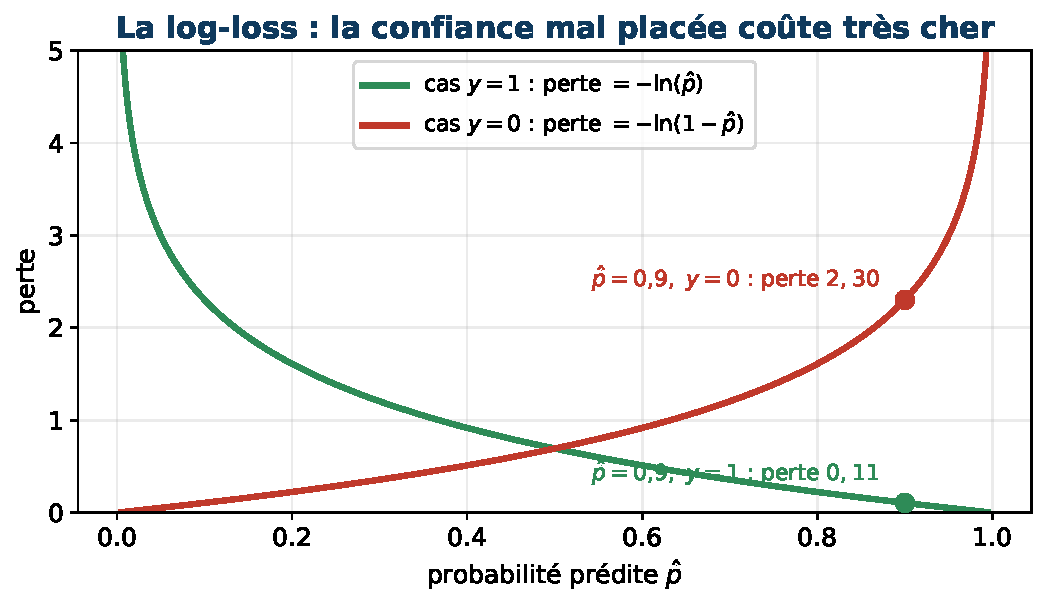
\includegraphics[width=\linewidth]{f6_logloss}
\end{columns}
\vspace{2pt}

{\small La bonne prédiction confiante coûte $0{,}105$ ; la même confiance, mal placée, coûte vingt-deux fois plus — et passer de $0{,}9$ à $0{,}99$ à tort \emph{double} encore la facture. La log-loss enseigne au modèle l'humilité : mieux vaut avouer $0{,}5$ que claironner une erreur.}
\end{frame}

\begin{frame}{Piège — parier 0 ou 1 : la perte infinie}
\begin{ucadpiege}[Pourquoi un modèle n'affirme jamais une certitude absolue]
{\small Prédire $\hat p = 1$ pour un patient finalement négatif coûte $-\ln(1-1) = -\ln 0 = +\infty$. Plus la probabilité s'approche des bords, plus une erreur devient ruineuse : $-\ln(0{,}1) = 2{,}30$, puis $-\ln(0{,}01) = 4{,}61$, puis $-\ln(0{,}001) = 6{,}91$, et ainsi de suite, sans limite.}
\end{ucadpiege}
{\small C'est précisément pour cela que la sigmoïde n'atteint \emph{jamais} exactement $0$ ni $1$ : elle met le modèle à l'abri de la catastrophe. Leçon pratique : une probabilité annoncée « en dur » à $0$ ou $1$ trahit presque toujours un bug (débordement numérique, division) plutôt qu'une vraie certitude — un classifieur sain reste prudent aux extrêmes.}
\end{frame}

\begin{frame}{Pas de solution exacte : la descente, encore}
\begin{ucaddef}[Ce qui change par rapport à la Séance 5]
{\small La log-loss n'a \textbf{pas d'équation normale} : aucune formule fermée ne donne ses meilleurs poids. Sa cuvette reste une vraie cuvette (un seul creux) — la \textbf{descente de gradient} de la Séance 5 s'applique donc telle quelle, et c'est ainsi que \texttt{LogisticRegression} s'entraîne.}
\end{ucaddef}
{\small Conséquences pratiques héritées de la Séance 5 :}
\begin{itemize}\small
  \item \texttt{max\_iter} plafonne le nombre de pas — l'avertissement \texttt{ConvergenceWarning} signifie « la descente n'avait pas fini » : augmenter \texttt{max\_iter}, et standardiser ;
  \item la \textbf{standardisation} (Séance 4) rend la cuvette ronde : \texttt{StandardScaler} \emph{puis} \texttt{LogisticRegression}, dans un Pipeline.
\end{itemize}
\end{frame}

\begin{frame}{L'aveu — \texttt{C}, la régularisation par défaut}
\begin{ucadpiege}[Un réglage caché dans les valeurs par défaut]
{\small \texttt{LogisticRegression} applique \textbf{d'office} une pénalité Ridge sur ses poids, dosée par \texttt{C} $= 1/\alpha$ : \emph{petit} \texttt{C} $=$ forte régularisation, \emph{grand} \texttt{C} $=$ faible. Le défaut \texttt{C}$\,= 1$ n'est pas neutre — c'est un choix.}
\end{ucadpiege}
{\small Sur le paludisme, l'effet est mesurable mais modeste ($5$ variables seulement) : \texttt{C}$\,=0{,}001$ écrase le plus grand poids à $0{,}32$ contre $0{,}75$ à \texttt{C}$\,=1$, pour une AUC quasi identique. Sur des problèmes plus riches, \texttt{C} devient décisif — son réglage \emph{propre} est l'affaire de la Séance 7.}
\end{frame}

\begin{frame}[fragile]{En pratique : LogisticRegression}
\begin{lstlisting}
from sklearn.pipeline import make_pipeline
from sklearn.preprocessing import StandardScaler
from sklearn.linear_model import LogisticRegression

modele = make_pipeline(StandardScaler(),
                       LogisticRegression(max_iter=1000, random_state=0))
modele.fit(X_train, y_train)
proba = modele.predict_proba(X_test)[:, 1]   # probabilites de la classe 1
y_pred = modele.predict(X_test)              # decision au seuil 0.5
\end{lstlisting}
{\small Deux sorties, deux usages : \texttt{predict\_proba} livre $\hat p$ (la matière première de toute la suite), \texttt{predict} applique le seuil $0{,}5$ — un raccourci dont la séance va montrer les limites.}
\end{frame}

\begin{frame}{Exercice — la log-loss à la main}
\begin{ucadrec}[Énoncé]
{\small Un modèle prédit $\hat p = 0{,}8$ pour deux patients. Le premier est réellement positif ($y=1$), le second négatif ($y=0$). Calculer la perte de chacun ($\ln 0{,}8 = -0{,}223$ ; $\ln 0{,}2 = -1{,}609$), puis la log-loss moyenne des deux.}
\end{ucadrec}
\pause
\begin{ucadex}[Correction]
{\small Patient 1 : perte $= -\ln 0{,}8 = \mathbf{0{,}223}$. Patient 2 : perte $= -\ln(1-0{,}8) = -\ln 0{,}2 = \mathbf{1{,}609}$ — sept fois plus cher. Moyenne : $(0{,}223 + 1{,}609)/2 = \mathbf{0{,}916}$. La même probabilité $0{,}8$ est un bon pari sur l'un, une faute lourde sur l'autre : la log-loss juge la prédiction \emph{face à la réalité}, jamais dans l'absolu.}
\end{ucadex}
\end{frame}

% #####################################################################
\section{La matrice de confusion}

\begin{frame}{L'idée : quatre façons d'avoir raison ou tort}
\begin{ucaddef}[L'idée en une phrase]
{\small Une décision binaire face à une réalité binaire ne peut tomber que dans \textbf{quatre cases} — deux succès, deux échecs — et ces quatre cases ne se valent pas : manquer un malade et alerter un bien-portant sont deux erreurs très différentes.}
\end{ucaddef}
\centering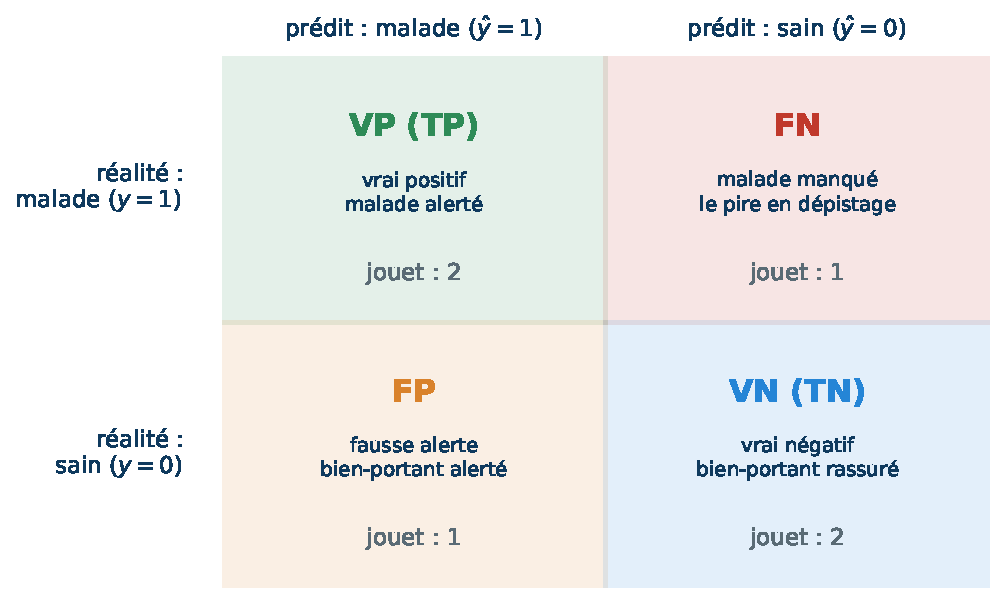
\includegraphics[width=0.52\linewidth]{f6_confusion}
\end{frame}

\begin{frame}{La matrice de confusion, formellement}
\begin{ucaddef}[Définition]
{\small La \textbf{matrice de confusion} croise réalité et prédiction : \textbf{TP} (vrais positifs), \textbf{FN} (faux négatifs : malades manqués), \textbf{FP} (faux positifs : fausses alertes), \textbf{TN} (vrais négatifs). Tout le reste de la séance n'est que des rapports entre ces quatre effectifs.}
\end{ucaddef}
\ucadformula{\text{TP} + \text{FN} = \text{nombre de positifs réels}\,, \qquad \text{TP} + \text{FP} = \text{nombre d'alertes émises}}
{\small Deux lectures de la même matrice : par \emph{ligne} (la réalité — où sont passés les malades ?) et par \emph{colonne} (la décision — que valent les alertes ?). Attention à la convention de \texttt{scikit-learn} : \texttt{confusion\_matrix} range les lignes par classe croissante, donc TN en haut à gauche.}
\end{frame}

\begin{frame}{Les quatre cases, en clair : quatre histoires}
\begin{ucadex}[Ce que chaque case signifie pour un patient réel]
{\small Sur le terrain, à Ziguinchor, les quatre cases sont quatre destins :
\begin{itemize}\small
  \item \textbf{TP} — un malade alerté, donc \emph{testé et soigné} : la mission réussie.
  \item \textbf{TN} — un bien-portant non alerté : \emph{rassuré} à juste titre, aucune ressource gaspillée.
  \item \textbf{FP} (fausse alerte) — un bien-portant alerté : il passe un test de confirmation \emph{pour rien} — coûteux, mais \textbf{récupérable}.
  \item \textbf{FN} (malade manqué) — un malade renvoyé chez lui sans soin : l'erreur la \textbf{plus grave}, parfois irréversible.
\end{itemize}
La leçon centrale de la séance tient là : FP et FN ne pèsent pas le même poids humain. Une métrique qui les \emph{additionne} — comme l'accuracy — efface précisément la distinction qui compte le plus.}
\end{ucadex}
\end{frame}

\begin{frame}{Exemple — le jouet des six patients}
\begin{ucadex}[Probabilités, décisions, matrice]
{\small Six patients, leurs probabilités prédites et la réalité — décision au seuil $0{,}5$ :
\begin{center}\footnotesize\renewcommand{\arraystretch}{1.05}\begin{tabular}{l|cccccc}
patient & $1$ & $2$ & $3$ & $4$ & $5$ & $6$\\\hline
$\hat p_i$ & $0{,}9$ & $0{,}75$ & $0{,}6$ & $0{,}4$ & $0{,}3$ & $0{,}1$\\
réalité $y_i$ & $1$ & $1$ & $0$ & $1$ & $0$ & $0$\\
décision $\hat y_i$ & $1$ & $1$ & $1$ & $0$ & $0$ & $0$\\
case & TP & TP & \textbf{FP} & \textbf{FN} & TN & TN\\
\end{tabular}\end{center}
Bilan : TP $= 2$, FP $= 1$, FN $= 1$, TN $= 2$. Le patient $3$ est une fausse alerte ; le patient $4$, un malade manqué. Ce jouet servira jusqu'à la courbe ROC.}
\end{ucadex}
\end{frame}

\begin{frame}{L'accuracy, revisitée}
\begin{ucaddef}[L'accuracy dans le langage de la matrice]
{\small L'accuracy de la Séance 3 est la diagonale des succès rapportée au total — elle additionne TP et TN \emph{comme s'ils se valaient}, et ignore la répartition des erreurs.}
\end{ucaddef}
\ucadformula{\text{accuracy} \;=\; \frac{\text{TP} + \text{TN}}{\text{TP} + \text{FP} + \text{FN} + \text{TN}} \;=\; \frac{2+2}{6} \;=\; 0{,}667 \quad \text{(jouet)}}
{\small Tant que les deux classes pèsent pareil, l'accuracy est un résumé honnête. Mais elle ne distingue pas un modèle qui manque des malades d'un modèle qui multiplie les fausses alertes — et sur une classe rare, elle deviendra carrément \textbf{menteuse}. Il faut des métriques qui regardent les cases une à une.}
\end{frame}

\begin{frame}{Precision et recall, formellement}
\begin{ucadfront}[Analogie]
{\small Un agent de santé communautaire fait du dépistage à Ziguinchor. Deux questions distinctes jugent son travail : \emph{quand il alerte, a-t-il raison ?} — et \emph{parmi les vrais malades du village, combien en a-t-il retrouvés ?} La première est la \textbf{precision}, la seconde le \textbf{recall}.}
\end{ucadfront}
\ucadformula{\text{precision} \;=\; \frac{\text{TP}}{\text{TP} + \text{FP}} \qquad\qquad \text{recall} \;=\; \frac{\text{TP}}{\text{TP} + \text{FN}}}
{\small La precision se lit sur la \emph{colonne} des alertes : la part d'alertes justifiées. Le recall se lit sur la \emph{ligne} des malades : la part de malades retrouvés. Chacune ignore ce que l'autre surveille — c'est ce qui rend leur couple si informatif.}
\end{frame}

\begin{frame}{Où se lisent precision et recall sur la matrice}
\centering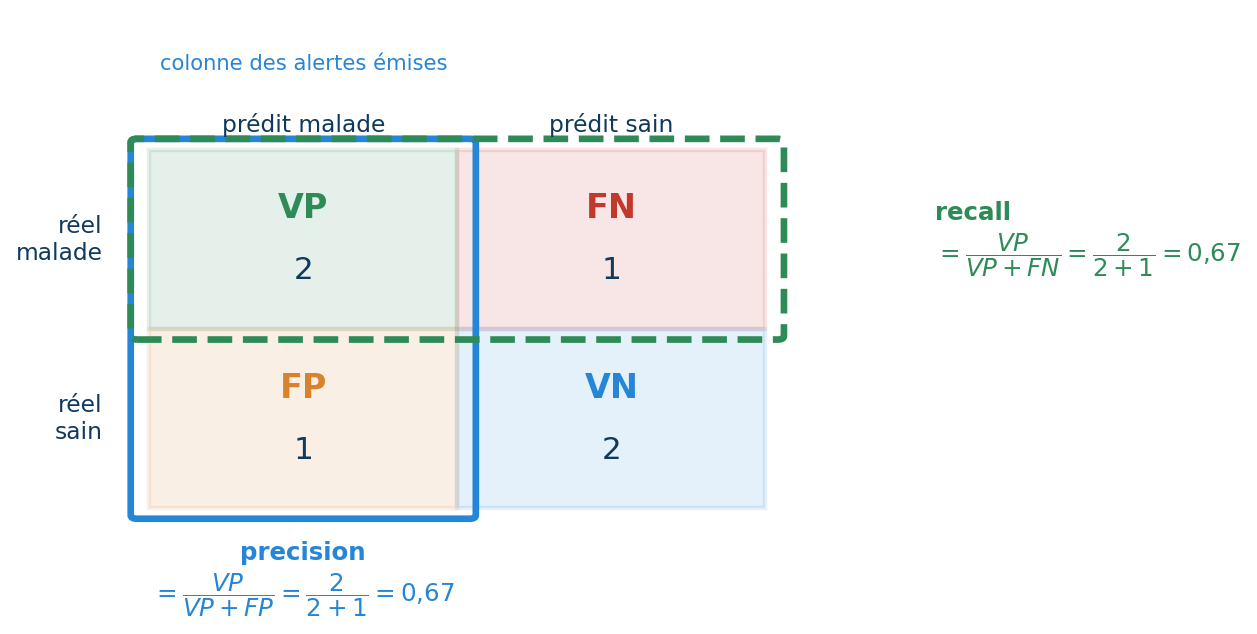
\includegraphics[width=0.64\linewidth]{f6_pr_matrix}
\vspace{-2pt}

{\small La même matrice, deux lectures. La \textbf{precision} (bleu) parcourt la \emph{colonne} des alertes : parmi tous les « malade ! » émis, combien étaient justes. Le \textbf{recall} (vert) parcourt la \emph{ligne} des vrais malades : parmi eux, combien ont été retrouvés. La case TP appartient aux \emph{deux} — c'est le succès que precision et recall se disputent. Et chacune ferme les yeux sur une case d'erreur différente : la precision oublie les FN, le recall oublie les FP.}
\end{frame}

\begin{frame}{Exemple — precision et recall du jouet}
\begin{ucadex}[Sur les six patients]
{\small Avec TP $= 2$, FP $= 1$, FN $= 1$ :
\[ \text{precision} = \frac{2}{2+1} = \mathbf{0{,}667} \qquad \text{recall} = \frac{2}{2+1} = \mathbf{0{,}667} \]
Deux alertes sur trois étaient justifiées ; deux malades sur trois ont été retrouvés. L'égalité est une coïncidence du jouet (FP $=$ FN) — en général les deux divergent, et c'est leur divergence qui raconte le comportement du modèle : beaucoup de FP tirent la precision vers le bas, beaucoup de FN tirent le recall.}
\end{ucadex}
\end{frame}

\begin{frame}{Piège — les deux métriques aux extrêmes}
\begin{ucadpiege}[Quand precision et recall se laissent berner]
{\small \textbf{N'alerter personne} (seuil très haut) : la precision vaut $\text{TP}/(\text{TP}+\text{FP}) = 0/0$, \emph{indéfinie} — \texttt{scikit-learn} renvoie $0$ assorti d'un avertissement. \textbf{Alerter tout le monde} (seuil nul) : le recall vaut $1$ trivialement, mais la precision s'effondre à la prévalence — sur le paludisme, $235/2000 = 0{,}12$. Chaque métrique, prise \emph{seule}, récompense une stratégie absurde.}
\end{ucadpiege}
{\small D'où la règle déjà posée : precision et recall ne se lisent qu'\textbf{ensemble} — et la F1, qui les marie par leur moyenne harmonique, refuse qu'on en sacrifie une pour gonfler l'autre.}
\end{frame}

\begin{frame}{La F1, formellement}
\begin{ucaddef}[Définition]
{\small La \textbf{F1} résume precision et recall en un seul nombre par leur \emph{moyenne harmonique} — une moyenne sévère, qui reste basse dès que \emph{l'une} des deux est basse.}
\end{ucaddef}
\ucadformula{F_1 \;=\; \frac{2\,\cdot\,\text{precision}\,\cdot\,\text{recall}}{\text{precision} + \text{recall}}}
{\small Jouet : $F_1 = \dfrac{2 \times 0{,}667 \times 0{,}667}{0{,}667 + 0{,}667} = \mathbf{0{,}667}$. Contre-exemple instructif : precision $= 1$ et recall $= 0{,}01$ donnent une moyenne arithmétique flatteuse de $0{,}505$, mais une F1 de $0{,}02$ — la moyenne harmonique refuse qu'une excellente precision \emph{achète} un recall misérable.}
\end{frame}

\begin{frame}{Exercice — une matrice à dépouiller}
\begin{ucadrec}[Énoncé]
{\small Sur $100$ patients de test : TP $= 8$, FP $= 2$, FN $= 4$, TN $= 86$. Calculer l'accuracy, la precision, le recall et la F1, puis dire en une phrase ce que ce modèle fait bien et ce qu'il fait moins bien.}
\end{ucadrec}
\pause
\begin{ucadex}[Correction]
{\small Accuracy $= 94/100 = \mathbf{0{,}94}$ ; precision $= 8/10 = \mathbf{0{,}80}$ ; recall $= 8/12 = \mathbf{0{,}667}$ ; $F_1 = \dfrac{2\times 0{,}80\times 0{,}667}{0{,}80+0{,}667} = \mathbf{0{,}727}$. Le modèle alerte à bon escient ($80\,\%$ d'alertes justifiées) mais \emph{manque un malade sur trois} — l'accuracy de $0{,}94$, aveuglée par les $86$ TN, ne laissait rien deviner de cette faiblesse.}
\end{ucadex}
\end{frame}

% #####################################################################
\section{Le seuil : un curseur, pas une constante}

\begin{frame}{Séparer prédire et décider}
\begin{ucaddef}[L'idée en une phrase]
{\small Le modèle produit des probabilités ; le \textbf{seuil} les transforme en décisions. Le baisser rend le modèle plus alarmiste (recall $\nearrow$, precision $\searrow$) ; le monter, plus prudent. Le seuil n'appartient pas au modèle : il appartient au \textbf{problème}.}
\end{ucaddef}
{\small Le $0{,}5$ par défaut suppose implicitement que les deux erreurs — manquer un malade, alerter un bien-portant — coûtent pareil. En santé publique, c'est presque toujours faux.}
\end{frame}

\begin{frame}{Analogie — le seuil, c'est une molette de sensibilité}
\begin{ucadfront}[Le détecteur de fumée]
{\small Un détecteur de fumée possède une molette de sensibilité. Réglée \textbf{haut}, l'alarme ne sonne que pour un vrai incendie : presque aucune fausse alerte (precision élevée), mais elle peut \emph{manquer} un départ de feu discret (recall faible). Réglée \textbf{bas}, elle sonne au moindre toast grillé : elle ne rate aucun feu (recall élevé) au prix de fausses alertes incessantes (precision basse). La molette ne change pas le \emph{détecteur} — elle choisit le \emph{compromis}.}
\end{ucadfront}
{\small Le seuil $s$ est exactement cette molette : le modèle et ses probabilités sont fixés, $s$ décide seulement à partir de quelle probabilité on déclenche l'alerte. Le régler, c'est répondre à une question de \textbf{coûts} — celui d'un malade manqué contre celui d'une fausse alerte — pas à une question de mathématiques.}
\end{frame}

\begin{frame}{Exemple — le jouet à seuil 0,35}
\begin{ucadex}[Les mêmes six patients, un autre seuil]
{\small Au seuil $0{,}35$, le patient $4$ ($\hat p = 0{,}4$) bascule en alerte :
\begin{center}\footnotesize\renewcommand{\arraystretch}{1.05}\begin{tabular}{l|cccccc}
patient & $1$ & $2$ & $3$ & $4$ & $5$ & $6$\\\hline
$\hat p_i$ & $0{,}9$ & $0{,}75$ & $0{,}6$ & $0{,}4$ & $0{,}3$ & $0{,}1$\\
réalité $y_i$ & $1$ & $1$ & $0$ & $1$ & $0$ & $0$\\
décision ($s=0{,}35$) & $1$ & $1$ & $1$ & $1$ & $0$ & $0$\\
\end{tabular}\end{center}
TP $= 3$, FP $= 1$, FN $= 0$ : precision $= 3/4 = \mathbf{0{,}75}$, recall $= 3/3 = \mathbf{1{,}0}$. Aucun paramètre du modèle n'a changé — seul le curseur a bougé, et le malade manqué a été rattrapé.}
\end{ucadex}
\end{frame}

\begin{frame}{La matrice se déforme quand le seuil descend}
\centering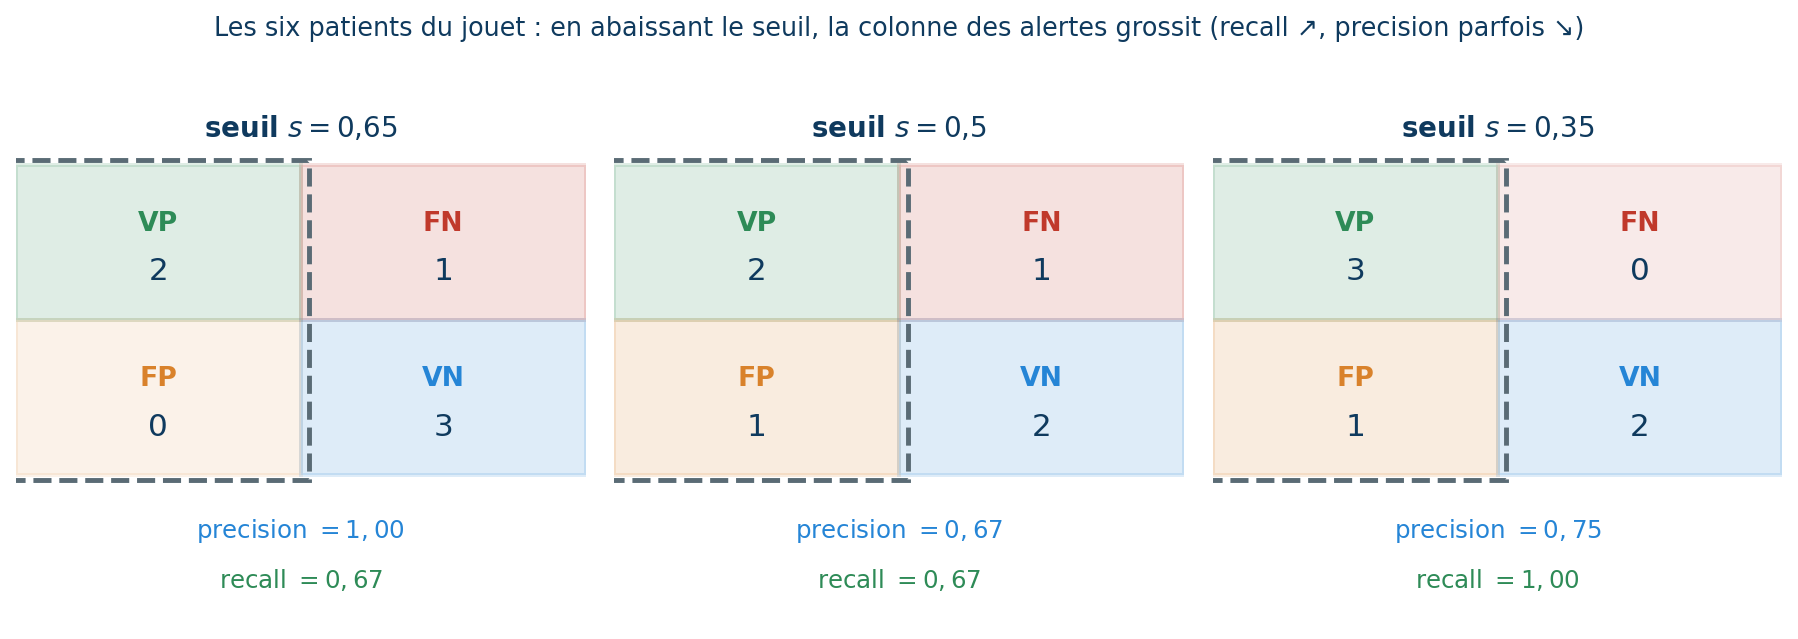
\includegraphics[width=0.86\linewidth]{f6_confusion_shift}
\vspace{-2pt}

{\small Les mêmes six patients, trois réglages de la molette. À $s = 0{,}65$, seules les deux alertes les plus sûres passent (precision parfaite, un malade manqué) ; en descendant à $0{,}35$, la \emph{colonne des alertes} se remplit : tous les malades sont rattrapés (recall $1{,}0$) au prix d'une fausse alerte. Le modèle reste \textbf{identique} — seul le curseur bouge.}
\end{frame}

\begin{frame}{Le paludisme au seuil 0,5 : personne}
\centering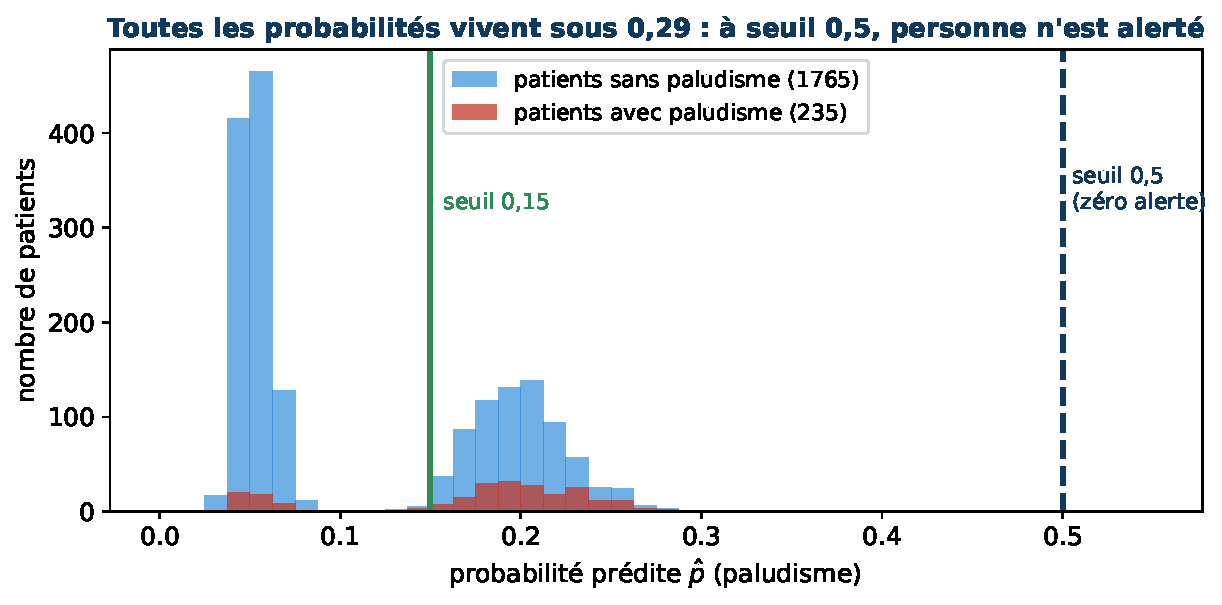
\includegraphics[width=0.60\linewidth]{f6_hist_proba}
\vspace{-2pt}

{\small Sur le test ($2\,000$ patients, $235$ malades), \textbf{toutes} les probabilités prédites vivent sous $0{,}29$ : au seuil $0{,}5$, zéro alerte, recall $= 0$, accuracy $= 0{,}8825 =$ la baseline. Le modèle \emph{semble} inutile — mais les malades (rouge) se concentrent à droite des bien-portants : le modèle \textbf{sépare}, c'est le seuil qui gaspille.}
\end{frame}

\begin{frame}{Le balayage chiffré}
\begin{ucadex}[Trois positions du curseur sur le paludisme]
{\small \begin{center}\renewcommand{\arraystretch}{1.1}\begin{tabular}{c|ccc|ccc}
seuil & TP & FP & FN & precision & recall & accuracy\\\hline
$0{,}5$ & $0$ & $0$ & $235$ & — & $0{,}00$ & $\mathbf{0{,}8825}$\\
$0{,}2$ & $100$ & $348$ & $135$ & $0{,}223$ & $0{,}426$ & $0{,}7585$\\
$0{,}15$ & $184$ & $720$ & $51$ & $0{,}204$ & $\mathbf{0{,}783}$ & $0{,}6145$\\
\end{tabular}\end{center}
À $0{,}15$, l'agent retrouve $78\,\%$ des malades au prix de $720$ fausses alertes — et l'accuracy \emph{chute}. Si la consigne est « ne pas laisser le paludisme circuler », le « pire » modèle au sens de l'accuracy est de loin le meilleur au sens de la mission.}
\end{ucadex}
\end{frame}

\begin{frame}{La courbe du compromis}
\centering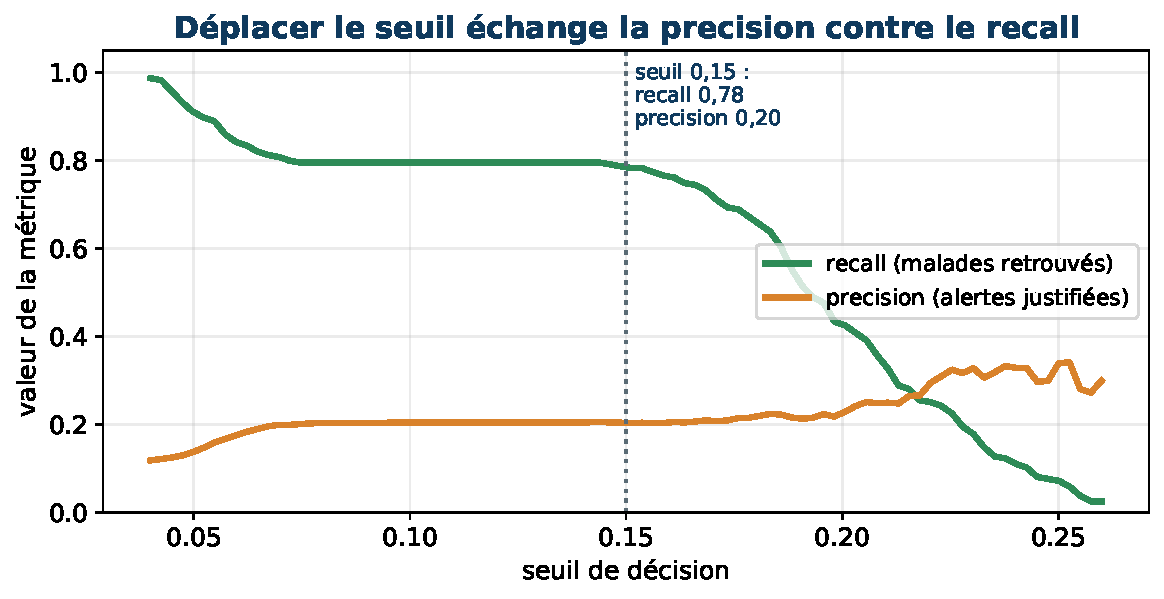
\includegraphics[width=0.74\linewidth]{f6_threshold}
\vspace{-2pt}

{\scriptsize Precision et recall en fonction du seuil : tout gain de l'une se paie sur l'autre. Le choix du point de fonctionnement est une décision de santé publique — coût d'un test de confirmation contre coût d'un malade manqué — pas une décision d'algorithme.}
\end{frame}

\begin{frame}{Exercice — precision et recall à deux seuils}
\begin{ucadrec}[Énoncé]
{\small Six patients, probabilités $\hat p = (0{,}9;\,0{,}7;\,0{,}45;\,0{,}4;\,0{,}35;\,0{,}3)$ et réalités $y = (1;\,0;\,0;\,1;\,0;\,0)$. Dresser la matrice de confusion au seuil $0{,}5$, puis au seuil $0{,}35$, et calculer precision et recall pour chacun. Que confirme la comparaison ?}
\end{ucadrec}
\pause
\begin{ucadex}[Correction]
{\small \textbf{Seuil $0{,}5$} : alertes sur les patients $1$ et $2$. TP $= 1$ (patient $1$), FP $= 1$ (patient $2$), FN $= 1$ (patient $4$), TN $= 3$ : precision $= 1/2 = \mathbf{0{,}50}$, recall $= 1/2 = \mathbf{0{,}50}$. \textbf{Seuil $0{,}35$} : alertes sur les patients $1$ à $5$. TP $= 2$, FP $= 3$, FN $= 0$, TN $= 1$ : precision $= 2/5 = \mathbf{0{,}40}$, recall $= 2/2 = \mathbf{1{,}0}$. Baisser le seuil a rattrapé le malade manqué (recall $0{,}50 \to 1{,}0$) mais multiplié les fausses alertes (precision $0{,}50 \to 0{,}40$) : le compromis, en chiffres.}
\end{ucadex}
\end{frame}

\begin{frame}{Exercice — choisir un seuil}
\begin{ucadrec}[Énoncé]
{\small Une campagne de dépistage à Kaolack dispose de tests de confirmation bon marché ; l'objectif sanitaire est de ne laisser passer presque aucun cas. Parmi les seuils $0{,}5$, $0{,}2$ et $0{,}15$ du balayage, lequel choisir, et quelle métrique faut-il accepter de sacrifier ?}
\end{ucadrec}
\pause
\begin{ucadex}[Correction]
{\small Seuil $\mathbf{0{,}15}$ : recall $0{,}783$, le seul compatible avec l'objectif « presque aucun cas manqué ». On sacrifie la precision ($0{,}204$ : quatre alertes sur cinq seront infirmées par le test de confirmation — acceptable puisqu'il est bon marché) et l'accuracy ($0{,}61$), qui n'a aucune pertinence ici. La métrique se choisit \emph{avant} le seuil, et toutes deux découlent du contexte.}
\end{ucadex}
\end{frame}

% #####################################################################
\section{ROC et AUC : juger le classement}

\begin{frame}{L'idée : juger toutes les positions du curseur à la fois}
\begin{ucaddef}[L'idée en une phrase]
{\small Plutôt que de juger le modèle \emph{à un seuil}, la courbe \textbf{ROC} le juge à \emph{tous} les seuils : elle trace, pendant que le curseur descend, la part de malades retrouvés (TPR $=$ recall) contre la part de bien-portants alertés à tort (FPR).}
\end{ucaddef}
\ucadformula{\text{TPR} \;=\; \frac{\text{TP}}{\text{TP}+\text{FN}} \qquad\qquad \text{FPR} \;=\; \frac{\text{FP}}{\text{FP}+\text{TN}}}
{\small TPR : le recall, déjà connu. FPR : son symétrique côté sains — la proportion de fausses alertes parmi les bien-portants. Le seuil maximal donne le point $(0,0)$ (aucune alerte) ; le seuil nul, le point $(1,1)$ (tout le monde alerté). Entre les deux, la courbe.}
\end{frame}

\begin{frame}{Le mécanisme — construire la ROC à la main (1/2)}
\begin{ucadex}[Trier puis descendre le curseur]
{\small Les six patients du jouet, \emph{triés} par probabilité décroissante ($3$ positifs, $3$ négatifs). On part du seuil le plus haut, puis on l'abaisse juste sous chaque $\hat p$ :
\begin{center}\footnotesize\renewcommand{\arraystretch}{1.08}\begin{tabular}{c|c|c|c|c}
le seuil passe sous & $y$ du patient & effet & TPR & FPR\\\hline
— (départ) & — & aucune alerte & $0/3$ & $0/3$\\
$0{,}9$ & $1$ & $+1$ TP $\Rightarrow$ \textbf{monter} & $1/3$ & $0/3$\\
$0{,}75$ & $1$ & $+1$ TP $\Rightarrow$ \textbf{monter} & $2/3$ & $0/3$\\
$0{,}6$ & $0$ & $+1$ FP $\Rightarrow$ \textbf{aller à droite} & $2/3$ & $1/3$\\
$0{,}4$ & $1$ & $+1$ TP $\Rightarrow$ \textbf{monter} & $3/3$ & $1/3$\\
$0{,}3$ puis $0{,}1$ & $0$, $0$ & $+2$ FP $\Rightarrow$ \textbf{à droite} & $3/3$ & $3/3$\\
\end{tabular}\end{center}
La règle tient en une ligne : en descendant la liste triée, chaque \textbf{positif fait monter}, chaque \textbf{négatif pousse à droite}.}
\end{ucadex}
\end{frame}

\begin{frame}{Le mécanisme — construire la ROC à la main (2/2)}
\centering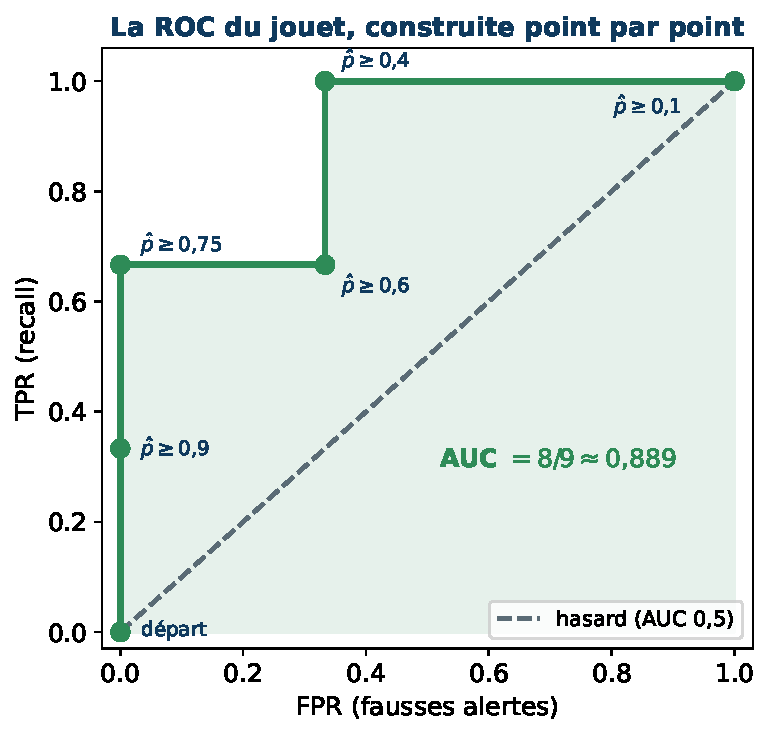
\includegraphics[width=0.40\linewidth]{f6_roc_toy}
\vspace{-2pt}

{\small Un modèle parfait monterait tout en haut avant de filer à droite (coin supérieur gauche) ; le hasard suivrait la diagonale. Le jouet ne commet qu'un faux pas : le patient $3$ (sain, $\hat p = 0{,}6$) classé au-dessus du patient $4$ (malade, $\hat p = 0{,}4$).}
\end{frame}

\begin{frame}{Exercice — lire TPR et FPR dans une matrice}
\begin{ucadrec}[Énoncé]
{\small À un seuil donné, un dépistage produit la matrice : TP $= 30$, FN $= 10$, FP $= 20$, TN $= 140$. Calculer le TPR (le recall) et le FPR, puis situer ce point sur la ROC : plutôt vers le bon coin, ou vers la diagonale ?}
\end{ucadrec}
\pause
\begin{ucadex}[Correction]
{\small TPR $= \dfrac{\text{TP}}{\text{TP}+\text{FN}} = \dfrac{30}{40} = \mathbf{0{,}75}$ : trois malades sur quatre retrouvés. FPR $= \dfrac{\text{FP}}{\text{FP}+\text{TN}} = \dfrac{20}{160} = \mathbf{0{,}125}$ : une fausse alerte pour huit bien-portants. Le point $(0{,}125\,;\,0{,}75)$ est nettement au-dessus de la diagonale (où un tirage au sort donnerait TPR $\approx$ FPR), donc bien orienté vers le coin supérieur gauche : un seuil de fonctionnement honnête.}
\end{ucadex}
\end{frame}

\begin{frame}{L'AUC, formellement}
\begin{ucaddef}[Définition]
{\small L'\textbf{AUC} (\emph{area under the curve}) est l'aire sous la courbe ROC — et elle possède une lecture probabiliste exacte : c'est la probabilité qu'un malade tiré au hasard reçoive une probabilité \emph{plus élevée} qu'un bien-portant tiré au hasard.}
\end{ucaddef}
\ucadformula{\text{AUC} \;=\; \frac{\text{nombre de paires (positif, négatif) bien ordonnées}}{\text{nombre total de paires}}}
{\small Jouet : $3 \times 3 = 9$ paires ; une seule est inversée (patient $3$ au-dessus du patient $4$) : AUC $= 8/9 \approx \mathbf{0{,}889}$ — exactement l'aire de l'escalier. Repères : $0{,}5 =$ hasard, $1 =$ classement parfait. L'AUC ne dépend d'\textbf{aucun seuil} : elle juge la qualité du \emph{tri}, rien d'autre.}
\end{frame}

\begin{frame}{L'AUC dépliée : les neuf paires du jouet}
\begin{ucadex}[Compter à la main les paires bien ordonnées]
{\small « Probabilité de bien ordonner une paire (malade, sain) » se vérifie à la main. Il y a $3$ malades ($\hat p = 0{,}9;\,0{,}75;\,0{,}4$) et $3$ sains ($\hat p = 0{,}6;\,0{,}3;\,0{,}1$), soit $3 \times 3 = 9$ paires. Une paire est \emph{bien classée} (\checkmark) si le malade reçoit la plus forte probabilité :
\begin{center}\footnotesize\renewcommand{\arraystretch}{1.25}
\begin{tabular}{c|ccc}
malade $\big\backslash$ sain & $0{,}6$ & $0{,}3$ & $0{,}1$\\\hline
$0{,}9$ & \checkmark & \checkmark & \checkmark\\
$0{,}75$ & \checkmark & \checkmark & \checkmark\\
$0{,}4$ & \textcolor{red}{\textbf{$\times$}} & \checkmark & \checkmark\\
\end{tabular}\end{center}
Huit paires sur neuf sont bien ordonnées ; l'unique faute est le malade à $0{,}4$, classé sous le sain à $0{,}6$. AUC $= 8/9 = \mathbf{0{,}889}$ — le même nombre que l'aire de l'escalier, obtenu en \emph{comptant les paires}.}
\end{ucadex}
\end{frame}

\begin{frame}{La ROC du paludisme : le verdict}
\centering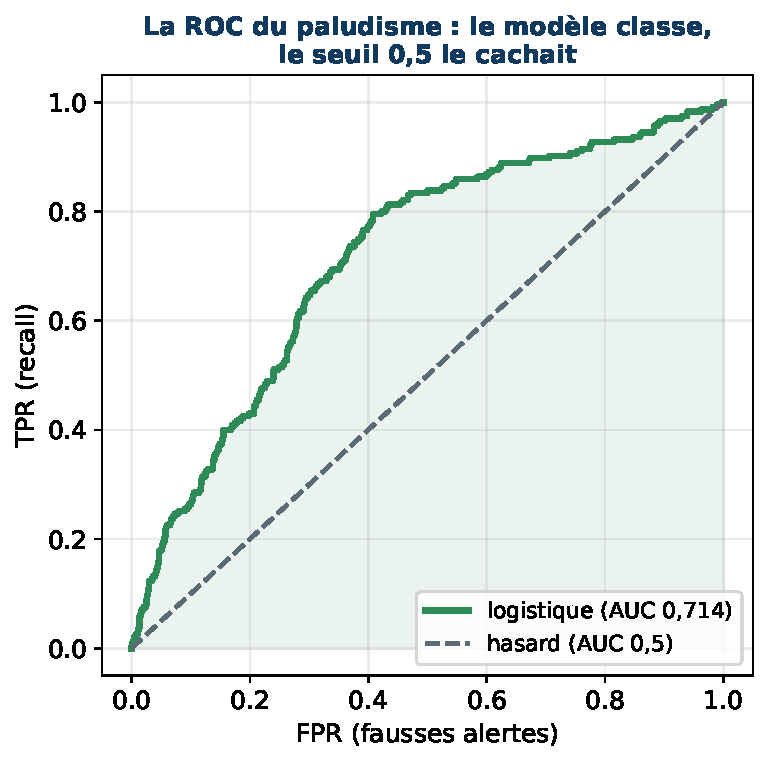
\includegraphics[width=0.38\linewidth]{f6_roc}
\vspace{-2pt}

{\small AUC $= \mathbf{0{,}714}$ : un malade pris au hasard est classé au-dessus d'un bien-portant pris au hasard $71\,\%$ du temps. Le modèle que l'accuracy déclarait inutile classe \textbf{nettement mieux que le hasard} : il fallait le juger sur le tri, puis choisir le seuil selon la mission.}
\end{frame}

\begin{frame}{Exercice — lire des AUC}
\begin{ucadrec}[Énoncé]
{\small Trois modèles de dépistage affichent AUC $= 0{,}50$, AUC $= 0{,}93$ et AUC $= 0{,}30$. Interpréter chacun — y compris le troisième, qui mérite réflexion.}
\end{ucadrec}
\pause
\begin{ucadex}[Correction]
{\small $0{,}50$ : le tri vaut un tirage au sort — modèle sans information. $0{,}93$ : excellent classement, un seuil utile existe sûrement. $0{,}30$ : le modèle classe \emph{systématiquement à l'envers} — pire que le hasard en apparence, mais il suffit d'\textbf{inverser ses prédictions} pour obtenir une AUC de $0{,}70$ : un tri constamment faux contient autant d'information qu'un tri constamment juste.}
\end{ucadex}
\end{frame}

% #####################################################################
\section{Le déséquilibre de classes}

\begin{frame}{La classe rare rend l'accuracy menteuse}
\centering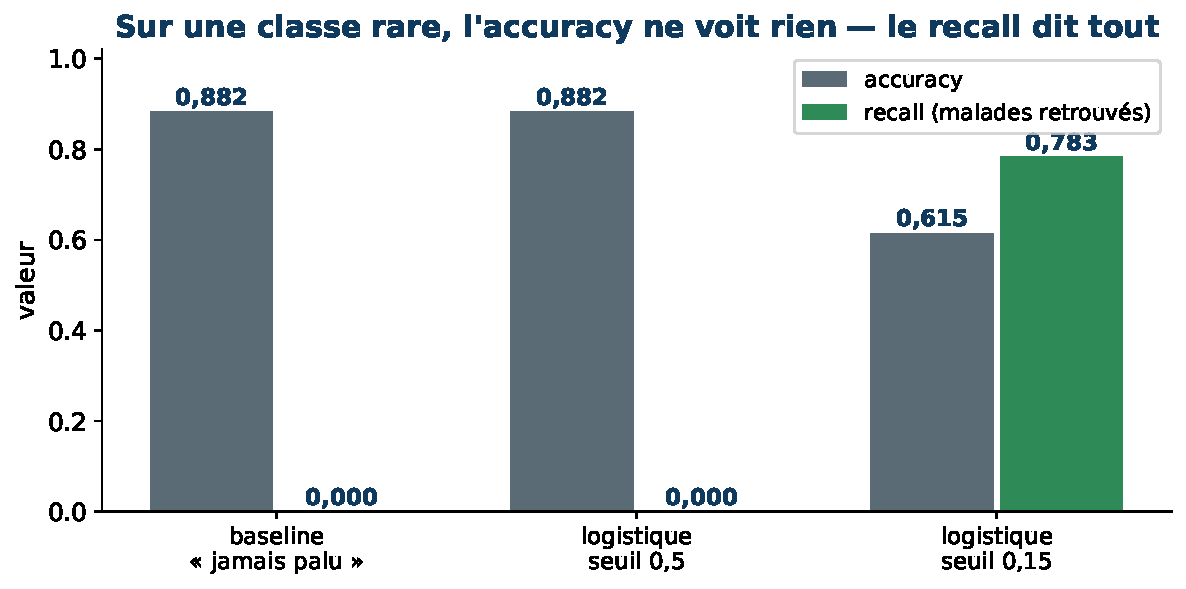
\includegraphics[width=0.70\linewidth]{f6_imbalance}
\vspace{-2pt}

{\small Avec $11{,}8\,\%$ de positifs, la baseline « jamais palu » affiche $0{,}8825$ d'accuracy sans rien savoir — un score que la logistique au seuil $0{,}5$ \emph{égale sans le battre}. Le recall démasque tout : $0$ et $0$ pour les deux premiers, $0{,}783$ au seuil $0{,}15$. Règle : sur classe rare, toute accuracy doit être comparée à celle de la baseline majoritaire — et accompagnée du recall.}
\end{frame}

\begin{frame}{Rééquilibrer l'entraînement : class\_weight}
\begin{ucaddef}[L'idée en une phrase]
{\small Plutôt que de déplacer le seuil \emph{après} l'entraînement, on peut corriger la log-loss \emph{pendant} : \texttt{class\_weight='balanced'} fait peser chaque malade autant que les $\approx 7{,}5$ bien-portants qu'il « représente », forçant le modèle à les prendre au sérieux.}
\end{ucaddef}
\begin{ucadex}[Effet chiffré sur le paludisme]
{\small Avec \texttt{class\_weight='balanced'} (seuil $0{,}5$ inchangé) : TP $= 187$, FP $= 727$, recall $= \mathbf{0{,}796}$, accuracy $= 0{,}6125$, AUC $= 0{,}715$. Le résultat est quasi identique au seuil $0{,}15$ du modèle standard — deux chemins (repondérer la perte, déplacer le curseur) vers le même compromis, et une AUC inchangée : le \emph{tri} n'a pas bougé, seule la décision.}
\end{ucadex}
\end{frame}

\begin{frame}{Quelle métrique pour quelle mission}
\begin{ucadret}[Le bon instrument selon l'objectif]
\begin{itemize}\small
  \item \textbf{Dépistage de masse} (manquer un cas coûte cher, confirmer est bon marché) : maximiser le \textbf{recall}, surveiller la precision.
  \item \textbf{Action coûteuse par alerte} (hospitalisation, traitement lourd) : privilégier la \textbf{precision}.
  \item \textbf{Comparer des modèles} indépendamment du seuil : \textbf{AUC} (et log-loss pour la qualité des probabilités).
  \item \textbf{Compromis unique demandé} : \textbf{F1}.
  \item \textbf{Accuracy} : seulement si les classes sont équilibrées \emph{et} les erreurs symétriques — sinon, jamais seule.
\end{itemize}
\end{ucadret}
\end{frame}

\begin{frame}{Exercice — la bonne métrique selon la mission}
\begin{ucadrec}[Énoncé]
{\small Associer à chaque situation la métrique à privilégier (recall, precision, AUC ou F1) : \textbf{(a)} comparer cinq modèles avant même d'avoir choisi un seuil ; \textbf{(b)} déclencher une chimiothérapie lourde et coûteuse sur la seule foi de l'alerte ; \textbf{(c)} dépister une épidémie où manquer un cas est dramatique et le test de confirmation est gratuit ; \textbf{(d)} rendre un unique chiffre de compromis dans un rapport.}
\end{ucadrec}
\pause
\begin{ucadex}[Correction]
{\small \textbf{(a)} \textbf{AUC} — elle juge le tri indépendamment du seuil, encore inconnu. \textbf{(b)} \textbf{precision} — chaque fausse alerte inflige un traitement lourd injustifié ; il faut que les alertes soient sûres. \textbf{(c)} \textbf{recall} — ne manquer aucun cas prime, et les fausses alertes sont rattrapées gratuitement. \textbf{(d)} \textbf{F1} — un seul nombre qui refuse de sacrifier l'une des deux. La métrique découle toujours du \emph{coût} des deux erreurs, jamais de l'habitude.}
\end{ucadex}
\end{frame}

\begin{frame}{Piège — régler le seuil sur le jeu de test}
\begin{ucadpiege}[Le curseur est un réglage comme un autre]
{\small Balayer les seuils \emph{sur le test} et garder le meilleur, c'est apprendre du test — la fuite de la Séance 4, déguisée. Le seuil (comme \texttt{C}) est un \textbf{hyperparamètre} : il se choisit sur des données de \emph{validation}, et le test ne sert qu'une fois, à la toute fin, pour le verdict.}
\end{ucadpiege}
{\small Reste une question que la séance laisse ouverte : comment réserver des données pour ces réglages sans appauvrir l'entraînement ? C'est exactement le problème que résout la \textbf{validation croisée} — Séance 7.}
\end{frame}

% #####################################################################
\section{Synthèse}

\begin{frame}{Le paludisme, enfin : l'arc en trois séances}
\begin{ucadex}[Trois tentatives, un dénouement]
{\small \begin{center}\renewcommand{\arraystretch}{1.12}\begin{tabular}{l|l|l}
séance & approche & verdict\\\hline
S3 & arbre, jugé à l'accuracy & $0{,}8825$ — ne bat pas la baseline\\
S5 & régression linéaire seuillée & $0{,}8825$ — zéro positif prédit\\
\textbf{S6} & logistique + bonnes métriques & AUC $\mathbf{0{,}714}$, recall $\mathbf{0{,}78}$ au seuil $0{,}15$\\
\end{tabular}\end{center}
La morale n'est pas « la logistique est meilleure que l'arbre » : c'est que les deux premières tentatives étaient jugées par une métrique \textbf{aveugle à la classe rare}. Changer d'instrument de mesure a fait apparaître la valeur qui était là.}
\end{ucadex}
\end{frame}

\begin{frame}{Le protocole de classification}
\begin{ucadret}[De bout en bout]
{\small \textbf{1.} Mesurer le déséquilibre (part de positifs) et poser la baseline majoritaire $\to$ \textbf{2.} split stratifié $\to$ \textbf{3.} Pipeline : \texttt{StandardScaler} puis \texttt{LogisticRegression} $\to$ \textbf{4.} récupérer les \textbf{probabilités} (\texttt{predict\_proba}), pas seulement \texttt{predict} $\to$ \textbf{5.} AUC pour juger le tri ; matrice de confusion, precision, recall au(x) seuil(s) candidats $\to$ \textbf{6.} choisir le seuil selon la \emph{mission} (sur validation, jamais sur test) $\to$ \textbf{7.} verdict final sur le test, métriques alignées avec l'objectif.}
\end{ucadret}
\end{frame}

\begin{frame}{À retenir — Séance 6}
\begin{ucadret}[L'essentiel]
\begin{itemize}\small
  \item La régression logistique $= $ le score linéaire de la Séance 5 $+$ la sigmoïde : une vraie \textbf{probabilité} en sortie, entraînée par \textbf{log-loss} et descente de gradient (pas de solution exacte).
  \item \textbf{Prédire} et \textbf{décider} sont deux étapes : le seuil transforme $\hat p$ en $\hat y$, et il appartient au problème, pas au modèle.
  \item La \textbf{matrice de confusion} décompose les erreurs ; \textbf{precision} (alertes justifiées) et \textbf{recall} (malades retrouvés) se lisent dedans ; la \textbf{F1} les résume sévèrement.
  \item La \textbf{ROC} juge tous les seuils à la fois ; l'\textbf{AUC} est la probabilité de bien ordonner une paire (malade, sain).
  \item Sur classe rare, l'\textbf{accuracy ment} : toujours la baseline majoritaire en référence, et le recall en regard.
  \item \texttt{C} régularise par défaut ; seuil et \texttt{C} sont des \textbf{hyperparamètres} — leur réglage propre arrive en Séance 7.
\end{itemize}
\end{ucadret}
\end{frame}

\begin{frame}{Pièges fréquents}
\begin{itemize}\small
  \item Annoncer une accuracy sur classe rare sans la baseline majoritaire en face.
  \item Confondre precision et recall — l'un juge les \emph{alertes}, l'autre les \emph{malades}.
  \item Garder le seuil $0{,}5$ par réflexe, comme s'il faisait partie du modèle.
  \item Régler le seuil (ou \texttt{C}) sur le jeu de test : c'est une fuite.
  \item Lire l'AUC comme une accuracy : elle parle de \emph{paires ordonnées}, pas de décisions.
  \item Oublier que \texttt{LogisticRegression} régularise par défaut (\texttt{C}$\,=1$) et exige la standardisation.
  \item Utiliser \texttt{predict} quand l'analyse demande \texttt{predict\_proba}.
\end{itemize}
\end{frame}

\begin{frame}{Prochaine séance}
\begin{ucadfront}[Séance 7 — Valider et régler sans tricher]
{\small La séance a laissé deux curseurs en suspens — le seuil et \texttt{C} — avec l'interdiction de les régler sur le test. La Séance 7 construit la solution : la \textbf{validation croisée}, les \textbf{grilles d'hyperparamètres} (\texttt{GridSearchCV}), et le protocole complet train / validation / test qui permet de régler sans se mentir.}
\end{ucadfront}
\end{frame}

\begin{frame}{Références}
\begin{itemize}\small
  \item James, Witten, Hastie, Tibshirani — \emph{An Introduction to Statistical Learning}, 2\textsuperscript{e} éd., Springer, 2021.
  \item Géron — \emph{Hands-On Machine Learning}, 3\textsuperscript{e} éd., O'Reilly, 2022.
  \item Müller, Guido — \emph{Introduction to Machine Learning with Python}, O'Reilly, 2016.
  \item Cours : University of Washington CSE 446 ; Stanford CS229.
\end{itemize}
\end{frame}

\end{document}
